\chapter{Máscara}


\section{Operações booleanas}

Após efetuar segmentações, é possível realizar operações booleanas entre as máscaras. As operações booleanas suportadas são:\\
\\
\textbf{União}, realiza a união de duas máscaras;\\
\textbf{Diferença}, realiza a diferença entre a primeira máscara com a segunda;\\
\textbf{Intersecção}, para apagar marcadores de objeto ou fundo.\\
\textbf{Disjunção exclusiva}, também é conhecida como XOR, mantém as regiões de ambas as máscara que possuem diferença.\\

Para ativar essa ferramenta é necessário ir no menu \textbf{Ferramentas}, \textbf{Operações boolenas}, como é exibido na figura~\ref{fig:booleano_menu} 

\begin{figure}[!htb]
\centering
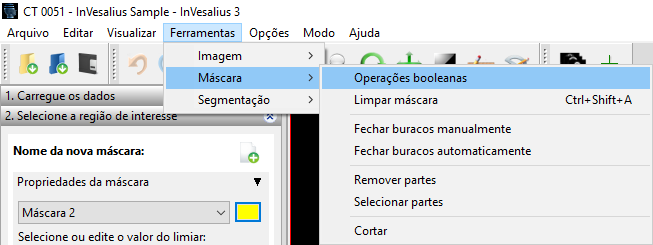
\includegraphics[scale=0.5]{mask_operation_boolean_menu_pt.png}
\caption{Menu para ativar a ferramenta de operações booleanas.}
\label{fig:booleano_menu}
\end{figure}

É necessário selecionar a primeira máscara, a operação a ser realizada e a segunda máscara conforme mostra a figura~\ref{fig:booleano_janela}. Em seguida é necessário clicar no botão \textbf{Ok}.

\begin{figure}[!htb]
\centering
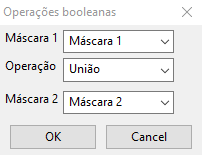
\includegraphics[scale=0.5]{mask_boolean_dialog_pt.png}
\caption{Ferramenta de operações booleanas.}
\label{fig:booleano_janela}
\end{figure}

Na figura~\ref{fig:op_boolana}, apresentamos um exemplo de utilização da ferramenta.

\begin{figure}[!htb]
  \centering
  \subfloat[Máscara A]{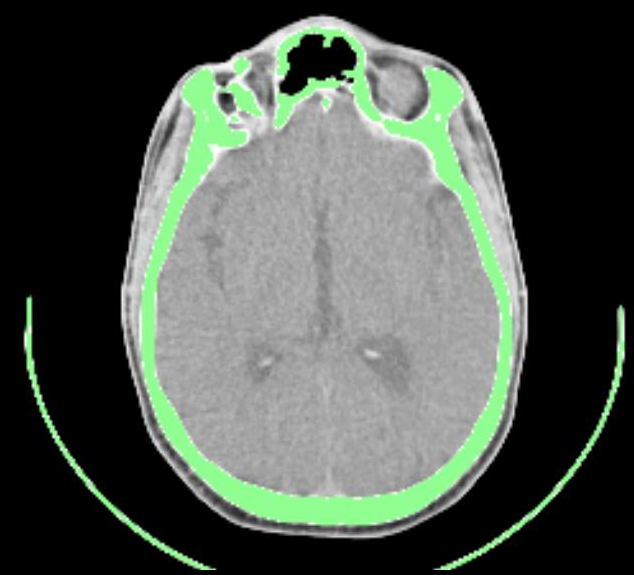
\includegraphics[width=0.332\textwidth]{booleano_m_a.png}}                
  \hfill
  \subfloat[Máscara B]{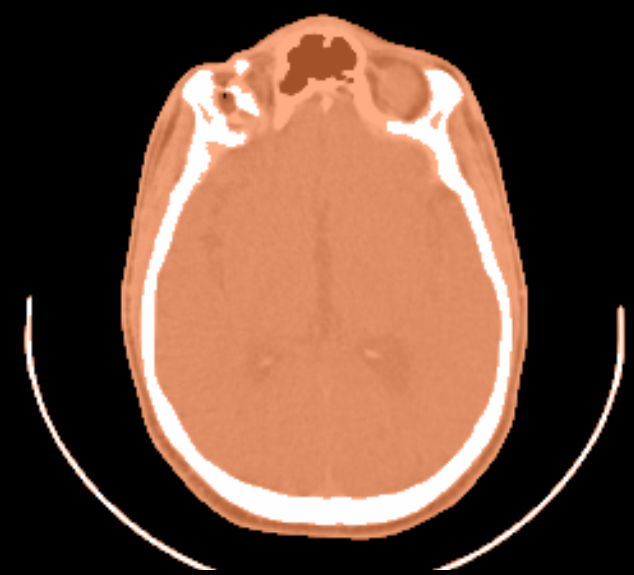
\includegraphics[width=0.332\textwidth]{booleano_m_b.png}}	
  \hfill  
  \subfloat[União (A $\cup$ B)]{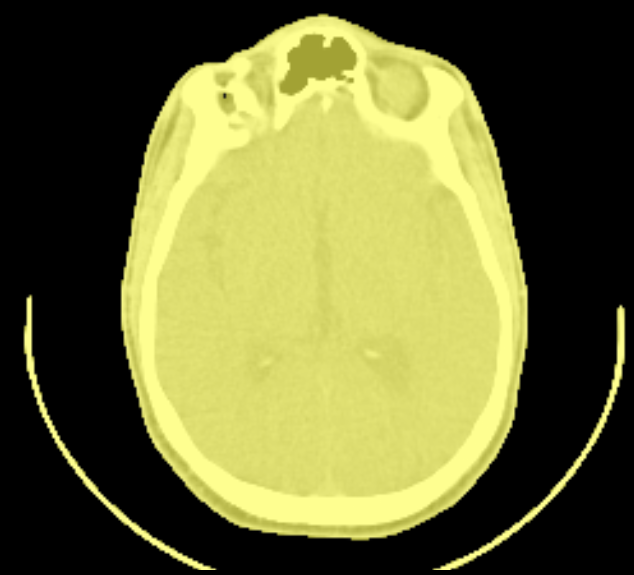
\includegraphics[width=0.332\textwidth]{booleano_uniao.png}}
  \hfill  
  \subfloat[Diferença (A - B)]{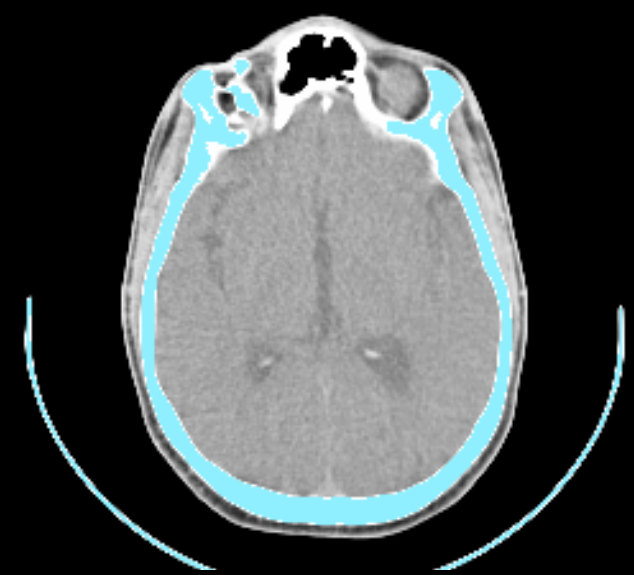
\includegraphics[width=0.332\textwidth]{booleano_dif.png}}
  \hfill  
  \subfloat[Intersecção (A $\cap$ B)]{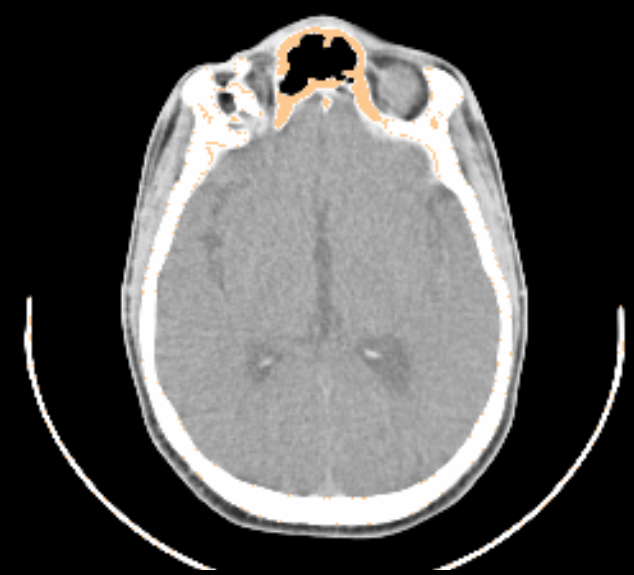
\includegraphics[width=0.332\textwidth]{booleano_interc.png}}
  \hfill  
  \subfloat[Disjunção exclusiva (A $\oplus$ B)]{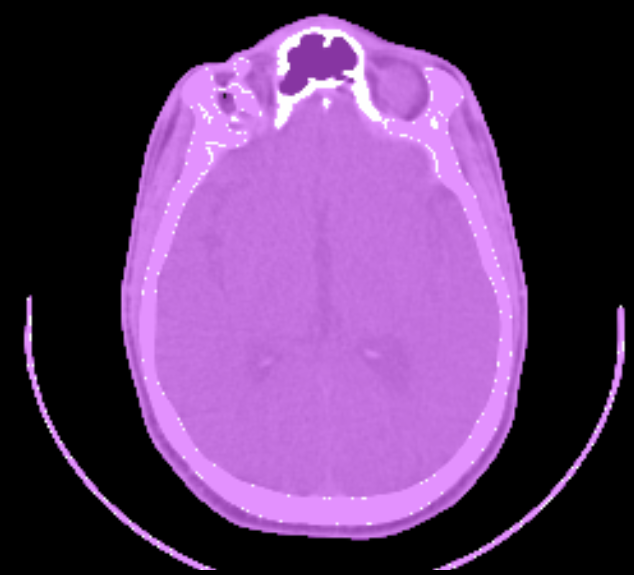
\includegraphics[width=0.332\textwidth]{booleano_disj_exc.png}}
  \caption{Exemplo de operações booleanas.}
  \label{fig:op_boolana}
\end{figure}

\section{Limpeza total da máscara}
\label{cap:limpeza_mascara}

Pode-se efetuar a limpeza total da máscara (figura~\ref{fig:limpeza_mascara}), isso é recomendado antes de iniciar a inserção de marcadores de Watershed. A ferramenta está localizada no menu, \textbf{Ferramentas}, \textbf{Máscara}, \textbf{Limpar máscara}, também é possível executa-la pressionando as teclas \textbf{CTRL+SHIFT+A}.

\begin{figure}[!htb]
\centering
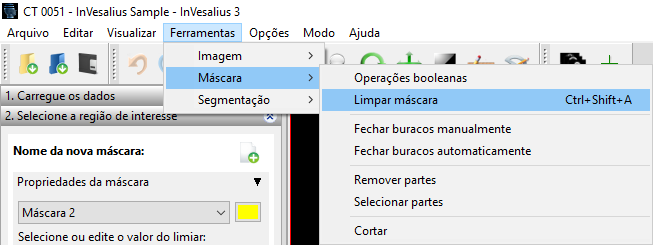
\includegraphics[scale=0.5]{mask_clean_menu_pt.png}
\caption{Limpeza de máscara}
\label{fig:limpeza_mascara}
\end{figure}